% !TEX encoding = UTF-8 Unicode
\documentclass[a4paper]{article}

\usepackage{color}
\usepackage{url}
\usepackage[T2A]{fontenc} % enable Cyrillic fonts
\usepackage[utf8]{inputenc} % make weird characters work
\usepackage{graphicx}

\usepackage[english,serbian]{babel}
%\usepackage[english,serbianc]{babel} %ukljuciti babel sa ovim opcijama, umesto gornjim, ukoliko se koristi cirilica

\usepackage[unicode]{hyperref}
\hypersetup{colorlinks,citecolor=green,filecolor=green,linkcolor=blue,urlcolor=blue}

\usepackage{listings}
\usepackage{amsthm}

%\newtheorem{primer}{Пример}[section] %ćirilični primer
%\newtheorem{primer}{Primer}[section]

\theoremstyle{definition}
\newtheorem{definition}{Definition}[section]

\definecolor{mygreen}{rgb}{0,0.6,0}
\definecolor{mygray}{rgb}{0.5,0.5,0.5}
\definecolor{mymauve}{rgb}{0.58,0,0.82}

\lstset{ 
  backgroundcolor=\color{white},   % choose the background color; you must add \usepackage{color} or \usepackage{xcolor}; should come as last argument
  basicstyle=\scriptsize\ttfamily,        % the size of the fonts that are used for the code
  breakatwhitespace=false,         % sets if automatic breaks should only happen at whitespace
  breaklines=true,                 % sets automatic line breaking
  captionpos=b,                    % sets the caption-position to bottom
  commentstyle=\color{mygreen},    % comment style
  deletekeywords={...},            % if you want to delete keywords from the given language
  escapeinside={\%*}{*)},          % if you want to add LaTeX within your code
  extendedchars=true,              % lets you use non-ASCII characters; for 8-bits encodings only, does not work with UTF-8
  firstnumber=1000,                % start line enumeration with line 1000
  frame=single,	                   % adds a frame around the code
  keepspaces=true,                 % keeps spaces in text, useful for keeping indentation of code (possibly needs columns=flexible)
  keywordstyle=\color{blue},       % keyword style
  language=Python,                 % the language of the code
  morekeywords={*,...},            % if you want to add more keywords to the set
  numbers=left,                    % where to put the line-numbers; possible values are (none, left, right)
  numbersep=5pt,                   % how far the line-numbers are from the code
  numberstyle=\tiny\color{mygray}, % the style that is used for the line-numbers
  rulecolor=\color{black},         % if not set, the frame-color may be changed on line-breaks within not-black text (e.g. comments (green here))
  showspaces=false,                % show spaces everywhere adding particular underscores; it overrides 'showstringspaces'
  showstringspaces=false,          % underline spaces within strings only
  showtabs=false,                  % show tabs within strings adding particular underscores
  stepnumber=2,                    % the step between two line-numbers. If it's 1, each line will be numbered
  stringstyle=\color{mymauve},     % string literal style
  tabsize=2,	                   % sets default tabsize to 2 spaces
  title=\lstname                   % show the filename of files included with \lstinputlisting; also try caption instead of title
}

\begin{document}

\title{Otkrivanje redudantnih test primera pomoću pokrivenosti koda\\ \small{Seminarski rad u okviru kursa\\Verifikacija softvera\\ Matematički fakultet}}

\author{Rastko Đorđević, Nikola Dimitrijević, Dimitrije Špadijer, Nadežda Bogdanović\\ kontakt email prvog, drugog, trećeg, nadezdabodanovic1@gmail.com}

%\date{9.~april 2015.}

\maketitle

\abstract{
Veliki problem, naročito kod softvera otvorenog koda i regresionog testiranja, predstavlja gomilanje redudantnih test primera i način njihovog otkrivanja. Naša definicija redudantnog test primera podrazumeva test primer, čijim  uklanjanjem iz skupa test primera pokrivenost linija koda ostaje neizmenjena. Pokrivenost koda merili smo alatom gcov i fokusirali smo se na test primere za QT framework. Cilj rada je da pojasni naš način implementacije otkrivanja redudantnih test primera. Rad ne sadrži formalne dokaze na kojima korektnost određenih postupka počiva, te se za te potrebe može koristiti predložena literatura.
}

\tableofcontents

\newpage

\section{Opis problema}
\label{sec:opis_problema}

Kod velikih projekata, primećuje se nagomilavanje test-primera, u čijem se međusobnom odnosu često primećuje visoka stopa redudantnosti. Međusobna redudantnost dva test-primera ukazuje na to da se svaka greška, koja se može naći jednim test-primerom, može naći i sa drugim i obrnuto.
Ovakva pojava ima ogromnog uticaja na efikasnost, vremnsku i prostornu, kao i na troškove samog testiranja.

Kako zbog politike vođenja samog projekta postoji velika sloboda dodavanja, a mala, ili gotovo nikakva provera prilikom dodavanja novih test-primera, ova pojava se posebno zapaža kod softvera otvorenog koda.

Ovakvome je softveru, zbog svoje prirode, potrebno dosta vremena kako bi stigao do završne faze svog razvojnog ciklusa, tako da je potrebno koliko god je moguće smanjiti trajanje svake od faza, a samim tim i testiranje.

\section{Opis rešenja}
\label{sec:opis_resenja}

Oslanjajući se na alat \textit{gcov} za merenje pokrivenosti koda, projekat koji smo odabrali kao prezentujući, pokrećemo najpre sa njegovim test primerima i merimo pokrivenost linija. Zatim uklanjamo jedan po jedan test primer, tako što ga jednostavno zakomentarišemo i merimo pokrivenost bez njega i ako ona ostaje nepromenjena, onda taj test primer označavamo kao redudantan.

Kao kriterijum pokrivenosti koristimo pokrivenost linija koda, zbog svoje intuitivne i prirodne interpretacije. Alat \textit{gcov} koristimo zato što je deo GNU ekosistema i kompatibilan je sa njegovim \textit{gcc} kompajlerom.

Da bismo mogli da uklonimo test primer iz skupa test primera, moramo najpre da ga pronađemo. Za te potrebe smo razvili parser i konteksno slbododnu gramatiku, koja je prilagodljiva različitim načinima generisanja test primera u okviru QT framework-a.

Odabrali smo testove generisane u okviru QT framework-a zbog njegove iskoristivosti na različitim platformama, a i zato što su naši članovi tima već upoznati za rad na takvoj platformi i njeno korišćenje im je udobno.

\subsection{Pseudokod osnovne ideje}
\label{subsec:pseudokod}
\begin{lstlisting}
getCoverage()
    compile project
    run tests
    generate coverage
    parse it and return metric
    
main()
    tests = {}
    
    for file in directory
        for test in file
            tests.add(test)
            
    baseline = getCoverage()
    
    for test in tests
        coverage = getCoverage()
        if coverage < baseline
            test.isRedudant = false
        else
            test.isRedudant = true
            
    print tests.filter(isRedudant)
\end{lstlisting}

\section{Opis arhitekture sistema}
\label{sec:arhitektura}

Osnovne komponente našeg rešenja objedinjene su u glavnom c++ fajlu, koji njima upravlja:
\begin{itemize}
    \item Komponenta za pronalaženje svih test-primera i njihovih lokacija:\\
            Svrha ovog modula je da pronađe sve test-primere u projektu i njihove lokacije, kako bi se mogli zakomentarisati, a počiva na integraciji c++ sa Flex-om (leksički analizator) i Yacc-om (parser). Ovo je moguće zato što Qt testovi moraju da se definišu na određeni način, tj. koriste određene ključne reči. Testove se traže rekurzivnom obilaskom direktorijuma u kojem se nalazi projekat koji se testira.
    \item Komponenta za komentarisanje i dekomentarisanje:\\
            Implementirana je kao bash skripta, zbog svoje konciznosti
    \item Komponenta za komunikaciju:\\
            Pisana je koristeći programski jezik Python i obuhvata sledeće akcije:
            \begin{itemize}
                \item Kompajliranje projekta koji se testira
                \item Izvršavanje kreiranih izvršnih fajlova
                \item Izvršavanje alata gcov, kako bi se izračunala pokrivenost
                \item Parsiranje izveštaja koji je kreirao gcov alat
                \item Vraćanje parsiranog rezultata glavnom programu
            \end{itemize}
    \item Komponenta koji pronalazi redudantnost:\\
            Vrši analizu i na osnovu prethodnodno dobijenih izveštaja i utvrđuje za svaki test-primer da li je redudantan u odnosu na ceo skup test-primera
\end{itemize}

\section{Pokretanje, rezultati i njihova procena}
\label{sec:pokretanje_rezultati_procena}

\subsection{Pokretanje i rezultati}
\label{subsec:pokretanje_rezultati}

\subsection{Prednosti:}
\label{subsec:prednosti}
\begin{itemize}
    \item Korišćenje je potpuno besplatno
    \item Pristup i tumačenje rezultata su intuitivni
    \item Nema lažno-negativnih (~eng. \textit{false negative}) rezultata: Ako neki test-primer nije označen kao negativan, onda to svakako nije
\end{itemize}

\subsection{Mane:}
\label{subsec:mane}
\begin{itemize}
    \item Mnogo lažno-pozitivnih rezultata: Ako je neki test-primer označen kao redudantan, ne znači nužno da to i jeste. Ovakav problem se javlja zato što se kao kriterijum pokrivenosti koristi pokrivenost linija.
    \item Nizak nivo skalabilnosti: Minimalan skup-test primera (onaj koji ne sadrži redudantnosti) se računa iznova i iznova za svako pokretanje. Ovo je posebno neefikasno za velike projekte.
    \item Velika zavisnost od izbora programskog jezika (podržava samo c++ projekte) i načina testiranja (podržava samo Qt testove) 
\end{itemize}


\section{Alternativna rešenja}
\label{sec:alternative}

Kao što je već pomenuto, rešenje koje smo odabrali, iako intuitivno, ima određene mane. One se mogu prevazići korišćenjem nekoliko različitih pristupa, od kojih smo mi odabrali dva najinteresantnija i prikazali ih u sekcijama koje slede.

\subsection{Otkrivanje redudantnih test-primera generisanih rešavačem modela primenom pokrivenosti koda}
\label{subsec:prvi}

Ovaj pristup\cite{prvinacin} podrazumeva da redudantnost znači da nema grešaka koje se mogu detektovati određenim test-primerom, a ne bez njega. Umesto da se redudantni testovi odbace, oni se transformišu tako da se redudantnost izbegne. Ovakav pristup nas oslobađa lažnih rezultata, a da pritom ne gubimo na pokrivenosti koda. Za generisanje, kao i za optimizaciju test primera koristi se proveravač modela (eng.~{\em model-checker}).

Da bismo utvrdili šta je test-primer, najpre moramo predstaviti pojam putanje.

\begin{definition}{Putanja:}
Putanja $ p := \{s_0, s_1, ...\}$ Kripke strukture $K$ je konačna ili beskonačna sekvenca takva da $ \forall i > 0 : (s_i, s_{i+1}) \in T za K, $ gde su $ s_i $ stanja modela.
\end{definition}

\begin{definition}{Test-primer (eng.~{\em test-case}):}
Test-primer $t$ je konačan prefiks putanje $p$ Kripke strukture $K$.
\end{definition}

Dužina test-primera: $ length(t) := i$ predstavlja broj svih stanja sa kojima test-primer dolazi u dodir.

\begin{definition}{Skup testova:}
Skup testova TS je konačan skup od n test-primera. Veličina skupa testova TS je n. Dužina skupa testova je zbir svih dužina njegovih test-primera: $
    length(TS) = \sum_{i=1}^{n}length(t_i)$
\end{definition}

Kao mera kvaliteta skupa test-primera koristi se kriterijum pokrivenosti modela. Takav kriterijum se može predstaviti kao skup osobina, gde test-primer pokriva određeni aspekt ako je odgovarajuća osobina narušena.

\begin{definition}{Pokrivenost testom:}
Pokrivenost C skupa testova TS, predstavljena skupom svojstava P je definisana kao odnos pokrivenog svojstva i ukupnog broja svojstava:
$
    C = \frac{1}{|P|}|{x|x \in P \land covered(x,TS)}|
$. Predikat $ covered(a, TS)$ je tačan ako postoji test-primer $ t \in TS$ takav da \em{t} pokriva \em{a}.
\end{definition}

Da bismo utvrdili da li su testovi redudantni, moramo najpre znati kako se izvršavaju:

\begin{definition}{Izvršavanje test-primera:}
Test-primer \em{t} za Kripke strukturu K se izvršava uzimanjem ulaznih varijabli svakog stanja, prosleđujući ih SUT-u sa odgovarajućim test-okvirom. Ove vrednosti i dobijene izlazne vrednosti predstavljaju putanju izvršavanja $ tr = \{s_{i}^{'}, s_{i+1}^{'}, ...\} $. Greška je detektovana akko $ \exists (s_{i}^{'}, s_{i+1}^{'}) \in tr : (s_{i}^{'}, s_{i+1}^{'}) \notin T za K $, gde se $ (s_{i}^{'}, s_{i+1}^{'})$ smatra za korak.
\end{definition}.

\subsubsection{Redudantnost u skupu testova}
\label{subsubsec:redudantnost}

Intuitivno, redudantni test-primeri su identični. Za svaka dva test-primera $t_1$, $t_2$, takvi da je $ t_1 = t_2$, svaka greška koja se može otkriti sa $t_1$, može se istovremeno otkriti i sa $t_2$ i obrnuto, pretpostavljajući da se oba test-primera izvršavaju sa istim preduslovima. Takođe, pokrivenost koju daje pokretanje test-primera $t_1$ jednako je pokrivenosti koju daje pokretanje $t_2$. Dolazimo do zaključka da skup testova nema potrebe za oba test-primera.

Do sličnog zapažanja se dolazi i u slučajevima kada je $t_1$ prefiks test-primera $t_1$, tako da se svaka greška koja se može detektovati sa $t_1$, može detektovati i sa $t_2$, ali ne i obprnuto. U ovom slučaju je $t_1$ redudantan i nije neophodan u onom skupu testova koji sadrži $t_2$.

Sve ovo prethodno dovelo nas je do redudantnosti za koju smo mi zainteresovani: Skup testova generisan pomoću rešavača modela je najčešće takav da svi test-primeri počinju istim inicijalnim stanjem. Počev od ovog stanja, može se prolaziti različitim putanjama, ali je mnogo putanja jednako nekom određenom stanju. Svaka greška koja se desi prilikom izvršavanja neke od ovih podputanji može biti detektovana bilo kojim test-primerom koji počinje ovom podputanjom. U sklopu ovih test-primera, podputanja je \textbf{redudantna}.

Ovakav pogled na redudantnost nam omogućava da skup test-primera predstavimo pomoću drveta, gde je inicijalno stanje, deljeno od strane svih test-primera koren drveta. Podputanja je redudantna ako se javlja u sklopu dva ili više test-primera. To znači da svaki čvor, osim inicijalnog, koji ima više od jedog deteta, sadrži redudantnost. Ako ima više različitih inicijalnih stanja, onda za svako od tih inicijalnih stanja postostoji po jedno drvo.

Dubina drveta jednaka je dužini najdužeg test-primera. Drvo izvršavanja se može koristiti za merenje redudantnosti.

\begin{definition}{Drvo izvršavanja skupa test-primera:}
Test-primer $t_i = \{s_0, s_1, ..., s_l\}$ iz skupa test-primera $TS$ se može pretstaviti kao drvo, gde je koren jednak inicijalnom stanju zajedničkom svim test-primerima: $root(TS) = s_0$. Za svaka dva uzastopna i različita stanja $s_i$ i $s_j$, gde $s_i$ prethodi stanju $s_j$, čvoru $s_i$ dodaje se dete $s_j$ na sledeći način: $s_j: (s_i, s_j) \in t_i \rightarrow s_j \in children(s_i)$.
\end{definition}

\begin{definition}{Redudantnost skupa test-primera:}
Redudantnost $R$ skupa test-primera $TS$ je definisana pomoću drveta izvršavanja:
\begin{equation}
\label{eq:suma}
    R(TS) = \frac{1}{n-1} \cdot \sum_{x \in children(root(TS))} \Re(x)
\end{equation}.
Redudantna vrednost $\Re$ za decu inicijalnog čvora se računa rekurzivnom formulom:
%\begin{equation}
%    \begin{cases}
%    (|children(x)-1|) + \sum_{c \in children(x)} \Re(c)  \cr  children(x) \neq %{} \\
%    0 \cr  children(x) = {} \\
%    \end{cases}
%\end{equation}
\end{definition}

\begin{verbatim}
\end{verbatim}

\begin{figure}[h!]
\begin{center}
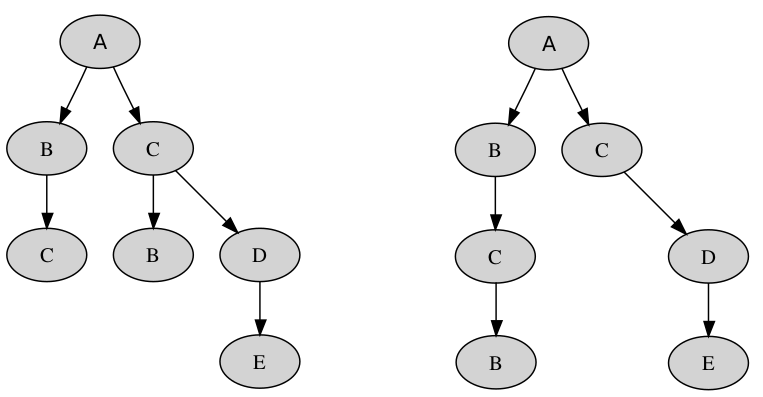
\includegraphics[scale=0.25]{redudancy.png}
\end{center}
\caption{Drvo sa redudantnošću od 17\% i drvo bez redudantnosti}
\label{fig:redudancy}
\end{figure}

Na slici \ref{fig:redudancy} prikazan je izgled drveta sa i bez redudantnosti. Postupak računanja procenta redudantnosti koristi formulu \ref{eq:suma}:
$ R = \frac{1}{7-1} \cdot (0 + (1+0)) = \frac{1}{6} = 17\% $.

Transformisanje test-primera iskače van domena ovog rada, pa ovde neće biti obrađeno, ali se detaljno objašnjenje može naći u literaturi\cite{prvinacin}.

\subsection{Otkrivanje redudantnosti test-primera analizom pokrivenosti koda}
\label{subsec:drugi}

Ovaj pristup\cite{druginacin} podrazumeva sledeće korake:
\begin{enumerate}
    \item \textbf{Nalaženje dijagrama toka:}\\
    Za program koji je pod testom, pronalazi se dijagram toka (~eng. \emph{control flow graph} - CFG). To znači da određeni testovi pobuđuju izvršavanje određenih delova koda, na osnovu kojih se formira CFG.
        \begin{figure}[h!]
        \begin{center}
        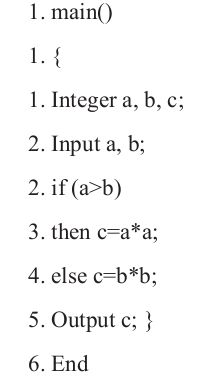
\includegraphics[scale=0.25]{program.png}
        \end{center}
        \caption{Program koji pronalazi veći od dva broja}
        \label{fig:program}
        \end{figure}
        Na slici \ref{fig:program} prikazan je program i za njega CFG, prikazan na slici \ref{fig:CFG}
        \begin{figure}[h!]
        \begin{center}
        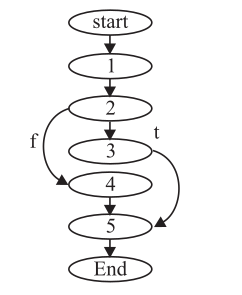
\includegraphics[scale=0.25]{CFG.png}
        \end{center}
        \caption{CFG datog programa}
        \label{fig:CFG}
        \end{figure}
    \item \textbf{Pronalaženje svih mogućih putanja iz CFG-a:}\\
        Na dijagramu \ref{fig:CFG} vidimo da su brojevima 1, 2, 3, 4, 5 označena stanja dijagrama toka, kao i početno (Start) i završno stanje (End). Takođe, primećujemo da u iz ovakvog dijagrama možemo ekstrahovati samo dve putanje: prvu koja prati nispunjenost uslova zadatog sa if i označićemo je kao $P_1$ i drugu koja prati izvršavanje u kojem uslov iz if nije ispunjen, označenu sa $P_2$.
    \item \textbf{Kreiranje matrice pokrivenosti:} \\
        Matrica pokrivenosti (putanja) povezuje testove i putanje sa kojima oni dolaze u dodir. Matrica po kolonama sadrži sve putanje, a po redovima sve testove. Informacija u matrici može biti '0' ili '1', gde '1' u i-tom redu i j-toj koloni znači da test-primer $t_i$ pobuđuje izvršavanje putanje $p_j$. Matrica pokrivenosti za naš primer predstavljena je na slici \ref{fig:pokrivenost}.
        \ref{fig:CFG}
        \begin{figure}[h!]
        \begin{center}
        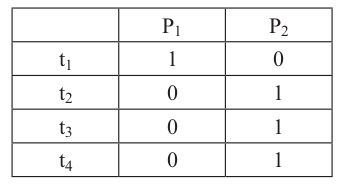
\includegraphics[scale=0.25]{Coverage.png}
        \end{center}
        \caption{Matrica pokrivenosti}
        \label{fig:pokrivenost}
        \end{figure}
    \item \textbf{Generisanje podskupova test-primera za odgovarajuće putanje}
    Za svaku putanju se generišu skupovi test-primera koji je pobuđuju, a na osnovu tog skupa i matrice pokrivenosti se računa i rezultat pokrivenosti (~eng. \textit{coverage score}) za svaki od test-primera po formuli: $ $
    Za naš primer koda, podaci se nalaze na slici
    \ref{fig:CFG}
        \begin{figure}[h!]
        \begin{center}
        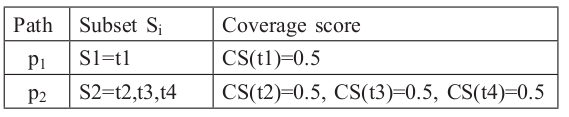
\includegraphics[scale=0.25]{Subsets.png}
        \end{center}
        \caption{Podskupovi test-primera}
        \label{fig:subtests}
        \end{figure}
    \item \textbf{Razlučivanje redudantnih i neredudantnih test-primera}
    Počevši od podskupa $S1$, primećujemo da on sadrži samo jedan test-primer $t_1$, te ga stavljamo u skup $TS_min$, koji predstavlja minimalni skup test-primtera koji nam je potreban. POsmatravši skup $S_2$, uviđamo da on sadrži testove čija je pokrivenost jednaka, što nas navodi na zaključak da su ovi testovi međusobno redudantni. Postavlja se pitanje: \emph{Koje od ovih testova ubaciti u minimalan skup test-primera?}
    \item \textbf{Razlučivanje korisnih od beskorisnih test-primera}
    Iako nije intuitivno, ovaj korak je ipak neophodan - on daje odgovor na prethodno pitanje. Možemo sada da izaberemo bilo koji test-primer koji će ući u minimalan skup test-primera koji nam je neophodan, a ostale da eleminišemo. Međutim, može se desiti situacija u kojoj se početni kod prepravi tako da ga test-primer koji smo odabrali ne pokriva i u tom slučaju on postaje beskoristan.
    
    Recimo da je, na slučajan način, u našem primeru izabaran $t_2$ tako da ulazi u skup $TS_{min}$. Sada je potrebno za test-primere $t_3$ i $t_4$ odrediti koji će u budućnosti biti koristan a koji ne. Kako oba test-primera prate putanju $P_2$, iz nje ćemo izvući uslove koji u njoj mogu da važe i oni će nam poslužiti kao kriterijum pri odlučivanju. Jedina dva moguća uslova su $c1_: a < b$ i $c2: a == b$. U ovom primeru je test $t_4$ takav da zadovoljava kriterijum $c_1$, ali ne i $c_2$, koji još uvek nije uključen u program. Test $t_3$ je takav da zadovoljava oba ova uslova, pa će on biti označen kao koristan i smešten u sekundarni skup test-primera $TS_{sec}$, koji je rezervi skup test-primera, a $t_4$ će, kako je redudantan i beskoristan biti potpuno odstranjen.
    
    Zaključno, primenom ovog postupka dobili smo minimalni skup test-primera koji nam je za sada potreban $TS_{min} = \{t_1, t_2\}$ i rezervni skup test-primera $TS_{sec} = \{t_3\}$ koji po potrebi može da nadopunjuje primarni skup.
\end{enumerate}

\section{Zaključak}
\label{sec:zakljucak}
Potpuno izbegavanje redudantnih test-primera je u velikim projektima jako teško i zbog toga se najčešće pribegava različitim tehnikama njihovog detektotavanja, a zatim i otklanjanja, ili transformisanja.

Postoji nekoliko načina koji obezbeđuju rešenje ovog problema. Pokazalo se u praksi da je jedan od najboljih ostvariv uz pomoć analize pokrivenosti koda. Te analize se mogu upotrebljavati na različite načine: korišćenje heuristika, statistika, rešavača modela, tabela pokrivenosti...

Ovakva rešenja su skalabilna i primenljiva i na druge skupove, a ne samo na skupove test-primera, te svoju primenu mogu naći i u biotehnologijama, statistici, i ostalim naučnim granama. Zbog toga se očekuje napredak istraživanja u ovoj oblasti paralelno sa napretkom gorepomenutih grana.

\addcontentsline{toc}{section}{Literatura}
\appendix
\bibliography{literatura} 
\bibliographystyle{plain}

\end{document}
